%****************************************************************
% Masters Thesis
% Created by 18/8/16
%
% Authors:
% Yang Jiang (jiangyang5157@gmail.com)
%
% This template is based on a template by:
% Vek (http://www.latextemplates.com/template/masters-doctoral-thesis) Version 2.3 (25/3/16)
% Steve Gunn (http://users.ecs.soton.ac.uk/srg/softwaretools/document/templates/)
% Sunil Patel (http://www.sunilpatel.co.uk/thesis-template/)
%
% Template license: CC BY-NC-SA 3.0 (http://creativecommons.org/licenses/by-nc-sa/3.0/)
%****************************************************************

%****************************************************************
%	CONFIGURATIONS
%****************************************************************
\documentclass[
	10pt, % The default document font size, options: 10pt, 12pt
	twoside, % Two side (alternating margins) for binding by default, uncomment to switch to one side
	chapterinoneline,% Have the chapter title next to the number in one single line
	english, % ngerman for German
	singlespacing, % Single line spacing, alternatives: onehalfspacing or doublespacing
	%draft, % Uncomment to enable draft mode (no pictures, no links, overfull hboxes indicated)
	%nolistspacing, % If the document is onehalfspacing or doublespacing, uncomment this to set spacing in lists to single
	liststotoc, % Uncomment to add the list of figures/tables/etc to the table of contents
	toctotoc, % Uncomment to add the main table of contents to the table of contents
	parskip, % Uncomment to add space between paragraphs
	%nohyperref, % Uncomment to not load the hyperref package
	headsepline, % Uncomment to get a line under the header
]{MastersDoctoralThesis} % The class file specifying the document structure

\usepackage[utf8]{inputenc} % Required for inputting international characters
\usepackage[T1]{fontenc} % Output font encoding for international characters
\usepackage{palatino} % Use the Palatino font by default

\usepackage[
	backend=bibtex,
	natbib=true,
	style=ieee,
	sorting=nyt
]{biblatex}

\addbibresource{Bibliographies/bibliography.bib} % The filename of the bibliography
\usepackage[autostyle=true]{csquotes} % Required to generate language-dependent quotes in the bibliography

\makeatletter
\def\blx@maxline{77}
\makeatother

%\usepackage[titletoc]{appendix}
%\usepackage[fleqn]{amsmath}
%\setlength{\mathindent}{10pt}
\usepackage{amsmath}
\usepackage{amssymb}
\usepackage{float}
\usepackage{multicol}
\usepackage{listings}
\usepackage[dvipsnames]{xcolor}

\lstdefinelanguage{Obj}{
	identifierstyle=\color{Black}\ttfamily\small,
	commentstyle=\color{Gray}\ttfamily\small,
	comment=[l]{\#},
	keywords={
		v,
		vn,
		f
	},
	keywordstyle=\color{Blue}\ttfamily\small\bfseries,
	sensitive=true
}

\lstdefinelanguage{Kml}{
	identifierstyle=\color{Black}\ttfamily\small,
	commentstyle=\color{Gray}\ttfamily\small,
	morecomment=[s]{<!--}{-->},
	keywords={
		http,
		https},
	keywordstyle=\color{Blue}\ttfamily\small\bfseries,
	morestring=[b]",
	stringstyle=\color{Green}\ttfamily\small,
 	sensitive=true
}

\lstdefinelanguage{Glsl}{
	identifierstyle=\color{Black}\ttfamily\small,
	commentstyle=\color{Gray}\ttfamily\small,
	comment=[l]{//},
	morecomment=[s]{/*}{*/},
	keywords={
		vec2,
		vec3,
		vec4,
		void,
		float,
		bool
	},
	keywordstyle=\color{Blue}\ttfamily\small\bfseries,
	ndkeywords={
		uniform,
		in,
		out,
		const
	},
	ndkeywordstyle=\color{orange}\bfseries,
	morestring=[b]",
	stringstyle=\color{Green}\ttfamily\small,
	sensitive=true
}

\lstdefinelanguage{Golang}{
	identifierstyle=\color{Black}\ttfamily\small,
	commentstyle=\color{Gray}\ttfamily\small,
	comment=[l]{//},
	morecomment=[s]{/*}{*/},
	keywords={
		nil,
		Handle,
		StripPrefix,
		FileServer,
		ListenAndServe
	},
	keywordstyle=\color{Blue}\ttfamily\small\bfseries,
	morestring=[b]",
	stringstyle=\color{Green}\ttfamily\small,
	sensitive=true
}

\lstdefinelanguage{Android}{
	identifierstyle=\color{Black}\ttfamily\small,
	commentstyle=\color{Gray}\ttfamily\small,
	comment=[l]{//},
	morecomment=[s]{/*}{*/},
	keywords={
		int,
		boolean,
		float,
		double,
		long,
		for,
		if,
		else
	},
	keywordstyle=\color{Blue}\ttfamily\small\bfseries,
	ndkeywords={
		return,
		new,
		private,
		protected,
		public,
		abstract,
		static,
		final,
		extends,
		implements
	},
	ndkeywordstyle=\color{orange}\bfseries,
	morestring=[b]",
	stringstyle=\color{Green}\ttfamily\small,
	sensitive=true
}

\lstset{
%title=\lstname, % show the filename of files included with \lstinputlisting; also try caption instead of title
%backgroundcolor=\color{white},
%frame=single, % adds a frame around the code: none, single, lines
%frame=trbl, % draw a frame at the top, right, left and bottom of the listing
%frameround=tttt, % make the frame round at all four corners
%framesep=4pt, % quarter circle size of the round corners
captionpos=b, % Position of the Caption (t for top, b for bottom)
extendedchars=true, % Allows 256 instead of 128 ASCII characters
columns=fixed, % make all characters equal width
keepspaces=true, % does not ignore spaces to fit width, convert tabs to spaces
tabsize=2, % number of spaces indented when discovering a tab
showstringspaces=false, % lets spaces in strings appear as real spaces
breaklines=true, % sets automatic line breaking
%numberstyle=\tiny\ttfamily
%numbers=left,% where to put the line-numbers; possible values are (none, left, right)
%numbersep=10pt, % how far the line-numbers are from the code
}

\setlength{\parskip}{\baselineskip}%
% Override line space
\linespread{1.4}

\geometry{ % Margins
	paper=a4paper, % Change to letterpaper for US letter
	bindingoffset=1.5cm,
	left=2.5cm,
	right=2.0cm,
	top=1.5cm, % Top margin
	bottom=1.5cm, % Bottom margin
	%showframe,% show how the type block is set on the page
}

\newcolumntype{C}[1]{>{\centering\let\newline\\\arraybackslash\hspace{0pt}}m{#1}}

%****************************************************************
%	INFORMATIONS
%****************************************************************
\thesistitle{Geographic Data Visualization with Immersive Virtual Reality} % Your thesis title, print it elsewhere with \ttitle
\keywords{Geographic Information,\;Visualization,\;Virtual Reality} % Keywords for your thesis, this is not currently used anywhere in the template, print it elsewhere with \keywordnames

\author{Yang \textsc{Jiang}} % Your name, print it elsewhere with \authorname
\supervisor{Dr Arno \textsc{Leist}} % Your supervisor's name, print it elsewhere with \supname

\university{\href{http://www.massey.ac.nz}{Massey University}} % Your university's name, print it elsewhere with \univname
\degree{\href{http://www.massey.ac.nz/massey/learning/programme-course-paper/programme.cfm?study_year=2016&prog_id=93070}{Master of Information Sciences}} % \degreename
\major{\href{http://www.massey.ac.nz/massey/learning/programme-course-paper/programme.cfm?study_year=2016&prog_id=93070&major_code=2363}{Software Engineering}} % \majorname
\paper{\href{http://www.massey.ac.nz/massey/learning/programme-course-paper/paper.cfm?study_year=2016&paper_code=159888}{159.888 Computer Science Professional Project}} % \papername

\hypersetup{pdftitle=\ttitle} % Set the PDF's title to your title
\hypersetup{pdfauthor=\authorname} % Set the PDF's author to your name
\hypersetup{pdfkeywords=\keywordnames} % Set the PDF's keywords to your keywords

%****************************************************************
%	BEGIN DOCUMENT
%****************************************************************
\begin{document}

%****************************************************************
%	FIRST PAGE
%****************************************************************
\frontmatter % Use roman page numbering style (i, ii, iii, iv...) for the pre-content pages
\pagestyle{plain} % Default to the plain heading style until the thesis style is called for the body content

\begin{titlepage}
\begin{center}
{\scshape\LARGE \univname\par}\vspace{1.5cm} % University name

\HRule \\[0.4cm] % Horizontal line
{\huge \bfseries \ttitle\par}\vspace{0.4cm} % Thesis title
\HRule \\[1.5cm] % Horizontal line

\vspace{2cm}

\begin{table}[H]
\centering
\large
\begin{tabular}{ C{5cm} C{5cm} }
\emph{Author} & \emph{Supervisor} \\
 {\authorname} & \href{http://www.massey.ac.nz/massey/expertise/profile.cfm?stref=359402}{\supname} \\
\end{tabular}\\[4cm]
\end{table}
 
\large \textit{A thesis submitted in fulfillment of the requirements\\ for the degree of \degreename}\\[0.2cm]
\textit{in the}\\[0.4cm]
\majorname\\\papername\\[2cm]
 
{\large \today}\\[4cm] % Date
%\includegraphics{massey-logo}
 
\vfill
\end{center}
\end{titlepage}

%****************************************************************
%	ABSTRACT PAGE
%****************************************************************
\begin{abstract}
\addchaptertocentry{\abstractname} % Add the abstract to the table of contents

Virtual reality technology has been proved to be beneficial to visualize geographic data. It can be broken down into the pseudo-3D display with 3D interaction and the immersible depth of vision of a real 3D experience. The former not only has been already studied for a long time in the domain of visualizing the earth and environmental sciences, but also got a favorable result in both theory and practice area. On the other hand, the latter is yet to be completely revealed. This paper makes a demonstrate of taking advantage of the Keyhole Markup Language (KML) \cite{google.kml.2016} as the geographic visualization markup language can not only benefit from the global geospatial group but contribute to all kind of communities. In consideration of the ranges any necessary sensors and the equipment costs, taking advantage of Google Cardboard \cite{google.cardboard.2016} and Android platform have proved to be well-suited for constructing the immersive virtual reality environment. This paper also revealed an immersive virtual reality based intuitive nature system that provides attractive and efficient methods for simultaneously visualizing geographic data from the different source. They are exposed by presenting the implementation of an virtual reality application that includes both front (client) and back-end (web server) for geographic data visualization. 

\end{abstract}

%****************************************************************
%	LIST OF CONTENTS
%****************************************************************
\setcounter{tocdepth}{2} % Exclude subsubsection in Contents
\tableofcontents % Prints the main table of contents

%****************************************************************
%	LIST OF FIGURES
%****************************************************************
\listoffigures % Prints the list of figures

%****************************************************************
%	LIST OF TABLES
%****************************************************************
\listoftables % Prints the list of tables

%****************************************************************
%	CHAPTERS
%****************************************************************
\mainmatter % Begin numeric (1,2,3...) page numbering
\pagestyle{thesis} % Return the page headers back to the "thesis" style

% Define some commands to keep the formatting separated from the content
\newcommand{\keyword}[1]{\textbf{#1}}
\newcommand{\tabhead}[1]{\textbf{#1}}
\newcommand{\code}[1]{\texttt{#1}}
\newcommand{\file}[1]{\texttt{\bfseries#1}}
\newcommand{\option}[1]{\texttt{\itshape#1}}
\newcommand{\norm}[1]{\lvert #1 \rvert} % Length of vector
\newcommand\tab[1][1cm]{\hspace*{#1}}

%****************************************************************
% Chapter X
%****************************************************************
\label{chapter-introduction}
\chapter{Introduction}

%****************************************************************
\section{Overview and Objectives}

The Geographic Information System (GIS) often refers to many different technologies, processes, and methods that designed to capture, store, manipulate, analyze, manage, and present spatial or geographical data \cite{wiki.gis.2016}. A GIS combines a database management system and a graphic display system that tie to the process of spatial analysis \cite{rhyne.virtual.1997}. Indeed, GIS has been widely used in the analysis of environmental data, but still significant problems have had exposed: first, GIS itself only handle 2D data; second, displays are limited to spatial views of the data; third, the capability of supporting user interaction with negligible data \cite{rhyne.visualization-gis.1994}. 

The Open Geospatial Consortium (OGC) is committed to making quality open standards for the global geospatial group. These standards were decided through a consensus based process and are freely available for anyone to sharing of the world's geospatial data. They have made contributions to many communities including government, commercial organizations, non-governmental organizations, academic and research organizations \cite{ogc.2016}. To use a markup language maintained by OGC for the creation of 3D geographic maps and associated spatial data allows scientists to publish the latest information in a single, simple data file format without technical assistance.

Since the technique progress in computers and the quick development in pipelined 3D graphics, GIS now can be used either with a workstation window based interface or with an immersive virtual reality environment \cite{koller.virtual-gis.1995}. In recent years, the immersive virtual reality not only frequent occurrences nearly in all sorts of media, but also it has explored a mess of related products. For example, immersive virtual reality headsets developed by manufacturers over the world, and the 3D camera that can capture a 360 degrees field of view. However, it is not mature enough to eliminate the equipment limitation and becomes a universal technology in daily life by comparison to the pseudo-3D virtual reality technology. For instance, when it comes to exploring, routing or getting to places, most people should just reach for Google Earth or Google Map.

There is a lack of research on visualizing geographic data in the immersive virtual reality environment. Therefore, we cannot yet say whether or not immersive virtual reality for geographic data visualization is better than other visualization and analysis approaches for certain data, if so, by how much; what basic considerations would be involved in immersive virtual reality based geographic data visualization. 

The purpose of this study are to explore how geographic data visualization with immersive virtual reality affect user interfaces and human-computer interactions; measure the ranges and capabilities of any necessary sensors; evaluate minimum equipment costs; takes advantage of the GIS and develop a virtual reality based geographic data visualization application including both front (client) and back-end (web server). In this thesis, a background of geographic data visualization is presented.  Then, details of the related technology and implementation in respect of the application are described. Finally, there is a discussion and conclusion around the results and future research.

%****************************************************************
\section{Background}
\label{section:background}

There has been an increased interest in the exploration of Virtual Environments (VE) \cite{huang.java-cgi-vr.2002}, sometimes called Virtual Reality (VR). Since beginning of 1990s when the development in the area of virtual reality became much more dynamic, and the term Virtual Reality itself became extremely popular, a wide range of applications were developed relatively fast, which offers significant benefits in many area, such as "architectural walkthrough", "scientific visualization", "modeling, designing and planning", "training and education", "telepresence and teleoperating", "cooperative working" and "entertainment" \cite{mazuryk.vr.1996}. Among these applications, virtual reality technology has been proved it offers new and exciting opportunities for users to interact visually with and explore 3D geo-data \cite{huang.java-cgi-vr.2002}.

In the past, GIS were mostly 2D, map-based systems, but the concept of taking advantage of GIS to visualize the earth and environmental sciences data has been already studied for a long time. That is called Virtual Globe (VG) technology, most of the virtual globe products use 3D representations of objects and display them onto a 2D monitor. This pseudo-3D nature of virtual globes allows users to interact in an environment that makes the data and information present easier to understand \cite{tuttle.virtual-globes.2008}. Then it has become a powerful tool for navigating geospatial data in 3D and contribute to all kind of communities across different usage till now. 

Given the current rapid development of virtual GIS technology, they made a point of the motivation of virtual reality technology is that people always want more, they want able to step into the world and interact with it, instead of watching the 2D projection image on the monitor. VR provides an easy used, powerful, intuitive way of user interaction. The user can experience and manipulate the simulated 3D environment in the same way they act in the real world, without any preparation or understanding of the complicated user interface works. It soon became a perfect tool that is beneficial to architects, designers, physicists, chemists, doctors, surgeons etc. Without a doubt VR has a great potential to change our life, the expectation from this technology is much more than it can offer yet. \cite{mazuryk.vr.1996} also discussed on an interesting idea that they came up with: new invention brings fear, the more potential it has, the bigger the danger can be.

The success of virtual globes \cite{tuttle.virtual-globes.2008} is not only because the improvement of human understanding from its pseudo-3D representations of objects and spaces, but also the five features: transportability (digital data are easily transported), scalability, interactivity (users are in control of the experience), choice of topics (topics can be combined or presented individually or ), currency (ability to adjust the data available to any given time period), and client-side \cite{tuttle.virtual-globes.2008}. Virtual globes can be beneficial to education ('For teaching spatial thinking, Virtual Globes offer tremendous opportunities, and it can be expected that they will greatly influence how a new generation will perceive space and geographical processes.' \cite{nuernberger.vr-classroom.2006}), scientific collaboration research (such as the EarthSLOT \cite{earthslot.2016}), and disaster response (VG is an invaluable tool in disaster response \cite{butler.vg.2006, nourbakhsh.mapping-disaster-zones.2006}). Virtual globe technology has many exciting possibilities for environmental science. The easy-to-use, intuitive nature system, provide attractive and effective means and methods for simultaneously visualizing four-dimensional environmental data from different sources that driving a greater understanding and user experience of the Earth system \cite{blower.sharing-visualizing.2007}. 

A markup language maintained by the Open Geospatial Consortium \cite{ogc.2016} plays an essential role in virtual reality implementation. By taking the use of a markup language, scientists are able to publish data in a single, simple data file format without technical assistance \cite{blower.sharing-visualizing.2007}. In spite of capabilities vary from products to products, but virtual globes always provide a support for a file format data exchange and the ability to simultaneously display multiple datasets. \cite{blower.sharing-visualizing.2007} points out Google Earth which has the largest community creates Keyhole Markup Language (KML) \cite{google.kml.2016} files as its primary method for visualizing data (KML is an international standard maintained by the OGC); NASA World Wind \cite{nasa.world-wind.2016} imports data from tile servers, OGC web services and a limited support for KML, it has more focus toward scientific users; ArcGIS Explorer \cite{esri.arcgis-explorer.2016} is a lightweight client to the ArcGIS Server, it can import data in a very wide range of GIS formats, including KML. Some of the virtual globes products are using Virtual Reality Modeling Language (VRML) \cite{wiki.vrml.2016} that is a language for describing 3D objects and interactive scenes on the World-Wide Web (WWW) \cite{wiki.www.2016}, It has been superseded by X3D \cite{wiki.x3d.2016}.

%Map is not only a tool for people getting from here to there but a way of organizing knowledge to make it understandable \cite{rhyne.visualization-gis.1994}.

%They also point out that map is not only a tool for people getting from here to there but a way of organizing knowledge to make it understandable.

%Visualization and GIS methodologies are often used to examine the Earth and environmental sciences data. 

%****************************************************************

%****************************************************************
% Chapter X
%****************************************************************
\label{chapter-technology}
\chapter{Technology}

%****************************************************************



%****************************************************************

%****************************************************************
% Chapter X
%****************************************************************
\label{chapter-implementation}
\chapter{Implementation}

%****************************************************************
\section{Google VR SDK}

%****************************************************************
\section{Scene}

%****************************************************************
\subsection{KML}

%****************************************************************
\subsection{Orctree}

%****************************************************************
\section{Earth}

The Earth is created as a UV Sphere, which somewhat like latitude and longitude lines of the earth, uses rings and segments. Near the poles (both on the Z-axis with the default orientation) the vertical segments converge on the poles. UV spheres are best used in situations where you require a very smooth, symmetrical surface.

\begin{figure}[H]
\caption[uv-sphere-mapping]{UV sphere mapping}
\label{fig:uv-sphere-mapping}
\centering
\includegraphics[width=\linewidth]{Figures/uv-sphere-mapping.png}
\decoRule
\end{figure}

As we can see the mapping from \ref{fig:uv-sphere-mapping}. Vertex $A0,\;A1,\;A2,\;A3,\;A4$ and $E0,\;E1,\;E2,\;E3,\;E4$ are duplicated, and $A0,\;B0,\;C0,\;D0,\;E0$ converge together as well as $A4,\;B4,\;C4,\;D4,\;E4$. So we can simply define it as a UV sphere has 5 rings and 4 segments. Also be noticed that each ring spans $2\,\pi$ radians, but each segment spans $\pi$ radians in the sphere mapping.

The total vertex number is:

\begin{equation}
\label{equ:uv-sphere-vertices}
Vertices = Rings \times Segments
\end{equation}

\begin{figure}[H]
\caption[uv-sphere-vertex]{UV sphere vertex}
\label{fig:uv-sphere-vertex}
\centering
\includegraphics[width=\linewidth]{Figures/uv-sphere-vertex.png}
\decoRule
\end{figure}

For each vertex $P$ on sphere from ring $r$ and segment $s$, we have:

\[
\begin{array}{lr}
v = r \times  \frac{1}{rings - 1} \\
u = s \times  \frac{1}{segments - 1} \\
\measuredangle \alpha = v \times \pi \\
\measuredangle \beta = u \times 2\,\pi \\
\end{array}
\]

$\therefore$ P (x,\;y,\;z)
\[
\begin{array}{lr}
x = (\sin(\alpha) \times radius) \times \cos(\beta) \\
y = \cos(\alpha) \times radius \\
z =  (\sin(\alpha) \times radius) \times \sin(\beta)
\end{array}
\]

$\And$ 2D Texture (x,\;y) mapping for vertex $P$ is:
\[
\begin{array}{lr}
x = u \\
y = v \\
\end{array}
\]

%****************************************************************
\section{Placemarker}

%****************************************************************
\subsection{Icosphere}

Generation of vertices for placemarker is a recursion process of subdividing icosphere. Figure \ref{fig:icosahedron-rectangles} shows that the initial vertices of an icosahedron are the corners of three orthogonal rectangles.

\begin{figure}[H]
\caption[icosahedron-rectangles]{Icosahedron rectangles \parencite{wiki.icosahedron-rectangles.2006}}
\label{fig:icosahedron-rectangles}
\centering
\includegraphics[width=\linewidth]{Figures/icosahedron-rectangles.png}
\decoRule
\end{figure}

Rounding icosphere by subdividing a face to an arbitrary level of resolution. One face can be subdivided into four by connecting each edge's midpoint.

\begin{figure}[H]
\centering
\includegraphics[width=\linewidth]{Figures/icosphere-subdivide.png}
\decoRule
\caption[icosphere-subdivide]{Icosphere subdivide}
\end{figure}

Then, push edge's midpoints to surface of the sphere.

\begin{figure}[H]
\centering
\includegraphics[width=\linewidth]{Figures/icosphere-refinement.png}
\decoRule
\caption[icosphere-refinement]{Icosphere refinement}
\end{figure}

\begin{table}[H]
\caption{Rounding Icosphere}
\label{tab:rounding-icosphere}
\centering
\begin{tabular}{l l l l}
\toprule
\tabhead{Recursion Level} & \tabhead{Vertex Count} & \tabhead{Face Count} & \tabhead{Edge Count} \\
\midrule
0 & 12 & 20 & 30 \\
1 & 42 & 80 & 120 \\
2 & 162 & 320 & 480 \\
3 & 642 & 1280 & 1920 \\
\bottomrule
\end{tabular}
\end{table}

%****************************************************************
\subsection{Geographic Coordinate System}

A geographic coordinate system is a coordinate system that enables every location on the Earth to be specified by a set of numbers or letters, or symbols \parencite{wiki.geographic-coordinate-system.2016}. A common geodetic-mapping coordinates is latitude, longitude and altitude (LLA), which also is the raw location data read from KML.

We introduce ECEF ("earth-centered, earth-fixed") coordinate system for converting  LLA coordinates to position coordinates. According to, the z-axis is pointing towards the north but it does not coincide exactly with the instantaneous earth rotational axis. The x-axis intersects the sphere of the earth at $0$ latitude and $0$ longitude \parencite{wiki.ecef.2016}.

\begin{figure}[H]
\centering
\includegraphics[width=\linewidth]{Figures/ecef.png}
\decoRule
\caption[ecef]{earth-centered, earth-fixed \parencite{wiki.ecef.2016}}
\end{figure}

The ECEF coordinates are expressed in a reference system that is related to mapping representations. Because the earth has a complex shape, a simple, yet accurate, method to approximate the earth’s shape is required. The use of a reference ellipsoid allows for the conversion between ECEF and LLA \parencite{u-blox.datum.1999}.

A reference ellipsoid can be described by a series of parameters that define its shape and which include a semi-major axis ($a$), a semi-minor axis ($b$), its first eccentricity ($e_1$) and its second eccentricity ($e_2$) as shown in Table \ref{tab:WGS-84-parameters}.

\begin{table}[H]
\caption{WGS 84 parameters}
\label{tab:WGS-84-parameters}
\centering
\begin{tabular}{l l l}
\toprule
\tabhead{Parameter} & \tabhead{Notation} & \tabhead{Value} \\
\midrule
Reciprocal of flattening & $1 / f$ & 298.257\,223\,563 \\
Semi-major axis & $a$ & 6\,378\,137\,m \\
Semi-minor axis & $b$ & $a\,(1 - f)$ \\
First eccentricity squared & $e_1^2$ & $1 - b^2 / a^2 = 2\,f - f^2$ \\
Second eccentricity squared & $e_2^2$ & $a^2 / b^2 - 1 = f\,(2 - f) / (1 - f)^2$ \\
\bottomrule
\end{tabular}
\end{table}

\begin{figure}[H]
\centering
\includegraphics[width=\linewidth]{Figures/ellipsoid-parameters.png}
\decoRule
\caption[ellipsoid-parameters]{Ellipsoid Parameters}
\end{figure}

The conversion from LLA to ECEF is shown below.

\begin{figure}[H]
\centering
\includegraphics[width=\linewidth]{Figures/lla2ecef.png}
\decoRule
\caption[lla2ecef]{LLA to ECEF}
\end{figure}

\[
\begin{array}{lr}
\begin{aligned}
x &= (N + h)\,\cos(\varphi)\,\cos(\lambda) \\
y &= (N + h)\,\cos(\varphi)\,\sin(\lambda) \\
z &= (\frac{b^2}{a^2}\,N + h)\,\sin(\varphi)
\end{aligned}
\end{array}
\]

Where

\[
\begin{array}{lr}
\begin{aligned}
\varphi &= \text{latitude} \\
\lambda &= \text{longitude} \\
h &= \text{height above ellipsoid (meters)} \\
N &= \text{Radius of Curvature (meters), defined as:} \\
&= \frac{a}{\sqrt{1 - e^2\,\sin(\varphi)^2}}
\end{aligned}
\end{array}
\]

At last, for this project usage, where high accuracy is not required, $a$ equals to $b$. And also the ECEF coordinate system is y-east, z-north (up), and x points to $0$ latitude and $0$ longitude, but for project specific, we still need to convert ECEF to x-east, y-north (up), and x points to $0$ latitude and $180$ longitude.

%****************************************************************
\subsection{Extra Model}

A simple and common OBJ format model can be loaded as an extra model for the placemarker.

%****************************************************************
\section{Textfield}

A textfield is a a rectangle vertices based renderable component to display text on a flat plane. Since it is a GL scene, the actual text will be drawn as a texture. By a constant width and native \code{android.text.StaticLayout} support, the height of the texture can be calculated. 

A menu contains multi-textfield can be seen as an empty textfield based which texture is fill full a pure background color, and several  textfields are laid out on the top of it with a certain vertical dimension.

A head rotation matrix (quaternion matrix \parencite{jvv.quaternions.2013}) is required for locating object in front of camera \parencite{mathworks.quaternion-rotation.2016} .

%****************************************************************
\section{Camera Movement}

In general, there are two sensors can be useful to manager camera movement: ACCELEROMETER (API level 3), LINEAR\_ACCELERATION (API level 9) and STEP\_DETECTOR (API level 19). 

LINEAR\_ACCELERATION is same as ACCELERATION which measures the acceleration force in meter per second repeatedly, except linear acceleration sensor is a synthetic sensor with gravity filtered out. 

\[
\begin{array}{lr}
Linear Acceleration = Accelerometer Data - Gravity \\
v = \int a\,dt \\
x = \int v\,dt
\end{array}
\]

First of all, we take the acclerometer data and remove gravity that is called gravity compensation, whatever is left is linear movement. Then we have to integrate it one to get velocity, integrated again to get position, which is called double integral. Now if the first integral creates drift, double integrals are really nasty that they create horrible drift. Because of these noise, using acceleration data it isn't so accurate, it is really hard to do any kind of linear movement \parencite{GoogleTechTalks.sensor-fusion.2010}.

On the other hand, use step counter from STEP\_DETECTOR, and pedometer algorithm for pedestrian navigation, that in fact works very well for this project.

\[
\begin{array}{lr}
p_1 = p_0 + v_0 \times dt \\
v_1 = v_0 + a \times dt
\end{array}
\]

The accuracy of this depends on how precision we can get for changing velocity. Considering that velocity is made of 3-axis directions, the current heading direction is required for a correct velocity calculation. Since the frame life cycle is implemented based on \parencite{Google.VR-SDK.2016}, which provide the heading direction in each frame callback. So I collect everything I need from the last frame to new frame, and update both velocity and position for each new frame.

For updating process, first of all, 

First of all, damping is required. I reduce velocity by a percentage. It is simply for avoiding that camear taking too long to stop. Damping by percentage can stable and stop the camera in a certain of time that won't be affected by the current camera speed. 


Secondly, a constant value in head forwarding direction is been used as a pulse for each step. Because a step is happening instantaneously which implies $a\,dt$ made by each step is actually can be replace by a constant value.

\begin{figure}[H]
\caption[camera-movement]{Camera movement}
\label{fig:camera-movement}
\centering
\includegraphics[width=\linewidth]{Figures/camera-movement.png}
\decoRule
\end{figure}

For each new frame:

\[
\begin{array}{lr}
\begin{aligned}
\overrightarrow{V_0} &= \overrightarrow{V_0} \cdot Damping \\
\overrightarrow{P_1} &= \overrightarrow{P_0} + \overrightarrow{V_0} \cdot dt \\
\overrightarrow{V_1} &= \overrightarrow{V_0} + \overrightarrow{Forwarding} \cdot Pulse \cdot Steps \\
Damping &\in [0,\enspace1] \\
Pulse &\in [0,\enspace \infty)
\end{aligned}
\end{array}
\]

%****************************************************************
\section{Ray Intersection}

Detect collisions between ray and models is the key to allow user selecting objects in the VR would, which is one of the importent experience for user interaction.

A ray can be describe in a equation with known ray start position \emph{$\overrightarrow{R_0}$} and ray direction \emph{$\overrightarrow{R_d}$}.

\begin{equation}
\label{equ:ray-t}
\overrightarrow{R(t)} = \overrightarrow{R_0} + \overrightarrow{R_d} \cdot t
\end{equation}

%****************************************************************
\subsection{Ray-Sphere}

\begin{figure}[H]
\caption[ray-sphere-intersection]{Ray-Sphere intersection}
\label{fig:ray-sphere}
\centering
\includegraphics[width=\linewidth]{Figures/ray-sphere-intersection.png}
\decoRule
\end{figure}

A point \emph{P} on the surface of sphere should match the equation:

\begin{equation}
\label{equ:sphere-surface}
(x_p - x_c)^2 + (y_p - y_c)^2 + (z_p - z_c)^2 = r^2
\end{equation}

If the ray intersects with the sphere at any position\emph{P} must match the equation \ref{equ:ray-t} and \ref{equ:sphere-surface}. Therefor the solution of \emph{t} in the cointegrate equation implies whether or not the ray will intersect with the sphere:

\[
\begin{aligned}
(x_{R_0} + x_{R_d} \cdot t - x_c)^2 &+ (y_{R_0} + y_{R_d} \cdot t - y_c)^2 + (z_{R_0} + z_{R_d} \cdot t - z_c)^2 = r^2 \\
&\vdots \\
x_{R_d}^2\,t^2 &+ (2\,x_{R_d}\,(x_{R_0} - x_c))\,t + (x_{R_0}^2 - 2\,x_{R_0}\,x_c + x_c^2) \\
+\;y_{R_d}^2\,t^2 &+ (2\,y_{R_d}\,(y_{R_0} - y_c))\,t + (y_{R_0}^2 - 2\,y_{R_0}\,y_c + y_c^2) \\
+\;z_{R_d}^2\,t^2 &+ (2\,z_{R_d}\,(z_{R_0} - z_c))\,t + (z_{R_0}^2 - 2\,z_{R_0}\,z_c + z_c^2) = r^2
\end{aligned}
\]

It can be seen as a quadratic formula:

\begin{equation}
\label{equ:sphere-surface-quadratic-formula}
a\,t^2 + b\,t + c = 0
\end{equation}

At this point, we are able to solved the \emph{t}:

\[
t =
\begin{cases}
\frac{-b \pm \sqrt{b^2 - 4\,a\,c}}{2\,a} & \text{if }\;b^2 - 4\,a\,c > 0 \\
\frac{-b}{2\,a} & \text{if }\; b^2 - 4\,a\,c = 0 \\
\varnothing & \text{if }\; b^2 - 4\,a\,c < 0
\end{cases}
\]

Then, I take a further step to get rid of formula complexity.

$\because$ Equation \ref{equ:sphere-surface},\,\ref{equ:sphere-surface-quadratic-formula}
\[
\left\{
\begin{array}{lr}
a = x_{R_d}^2 + y_{R_d}^2 + z_{R_d}^2 \\
b = 2\,(x_{R_d}\,(x_{R_0} - x_c) + y_{R_d}\,(y_{R_0} - y_c) + z_{R_d}\,(z_{R_0} - z_c)) \\
c = (x_{R_0} - x_c)^2 + (y_{R_0} - y_c)^2 + (z_{R_0} - z_c)^2 - r^2
\end{array}
\right.
\]

$\And$
\[
\begin{array}{lr}
\begin{aligned}
\norm{\overrightarrow{R_d}} &= \sqrt{x_{R_d}^2 + y_{R_d}^2 + z_{R_d}^2} = 1 \\
\overrightarrow{V_{c\_R_0}} &= \overrightarrow{R_0} - \overrightarrow{C} = \overrightarrow{(x_{R_0} - x_c,\enspace y_{R_0} - y_c,\enspace z_{R_0} - z_c)}
\end{aligned}
\end{array}
\]

$\therefore$
\[
\left\{
\begin{array}{lr}
a =1 \\
b = 2 \cdot \overrightarrow{R_d} \cdot \overrightarrow{V_{c\_R_0}} \\
c = \overrightarrow{V_{c\_R_0}} \cdot \overrightarrow{V_{c\_R_0}} \cdot r^2
\end{array}
\right.
\]

$\because$ The formula for \emph{t} can also be optimized
\[
\left\{
\begin{array}{lr}
\frac{-b \pm \sqrt{b^2 - 4\,a\,c}}{2\,a} = -\alpha \pm \sqrt{\beta} \\
\alpha = \frac{1}{2}\,b \\
\beta = \alpha^2 - c
\end{array}
\right.
\]

$\therefore$ The final solution for \emph{t}
\[
t =
\begin{cases}
 -\alpha \pm \sqrt{\beta} & \text{if }\;\beta > 0 \\
-\alpha & \text{if }\;\beta = 0 \\
\varnothing & \text{if }\;\beta < 0
\end{cases}
\]

And the collision position for each \emph{t} is:

\[
\overrightarrow{P} = \overrightarrow{R_0} + \overrightarrow{R_d} \cdot t
\]

%****************************************************************
\subsection{Ray-Plane}
\parencite{stackoverflow.ray-plane.2014} \\

\begin{figure}[H]
\caption[ray-plane-intersection]{Ray-Plane intersection}
\label{fig:ray-plane}
\centering
\includegraphics[width=\linewidth]{Figures/ray-plane-intersection.png}
\decoRule
\end{figure}

If a point \emph{P} on the plane and also belongs to the ray, we have quadric equation:

\begin{equation}
\label{equ:ray-plane-intersection}
\left\{
\begin{array}{lr}
(\overrightarrow{P} - \overrightarrow{P_1}) \cdot \overrightarrow{N} = 0 \\
\overrightarrow{P} = \overrightarrow{R_0} + \overrightarrow{R_d} \cdot t
\end{array}
\right.
\end{equation}

Solution for the \emph{t} is:

\[
t =
\begin{cases}
\frac{-\overrightarrow{N} \cdot (\overrightarrow{R_0} - \overrightarrow{P_1})}{\overrightarrow{N} \cdot \overrightarrow{R_d}} & \text{if }\;\overrightarrow{N} \cdot \overrightarrow{R_d} \nsim 0 \\
\varnothing & \text{if }\;\overrightarrow{N} \cdot \overrightarrow{R_d} \sim 0
\end{cases}
\]

At last, we have to verify if the collision is inside of the quadrangle by putting \emph{t} back to \ref{equ:ray-plane-intersection}, and the \emph{t} is valid only if:

\[
\begin{array}{lr}
\mu = \sqrt{(\overrightarrow{P} - \overrightarrow{P_1}) \cdot (\overrightarrow{P_2} - \overrightarrow{P_1}))} \in [0,\enspace\norm{\overrightarrow{P_2} - \overrightarrow{P_1}}] \\
\nu = \sqrt{(\overrightarrow{P} - \overrightarrow{P_1}) \cdot (\overrightarrow{P_3} - \overrightarrow{P_1}))} \in [0,\enspace\norm{\overrightarrow{P_3} - \overrightarrow{P_1}}] 
\end{array}
\]

%****************************************************************
\subsection{Ray-Box}
\parencite{Williams.ray-box.2005} \\
\parencite{Tavian.ray-box-2d.2011} \\
\parencite{scratchapixel.ray-plane-3d} \\

There is a octree implementation in the VR 3D world that separate the 3D world to invisible 3D boxes that each box contains a certain number of other models. It is to avoid unnecessary ray-object collision detection. In this section, I am going to first explain Ray-Box-2D collision detection, then derive out Ray-Box-3D intersection.

%****************************************************************
\subsubsection{Ray-Box-2D}

\begin{figure}[H]
\caption[ray-box-2d-intersection]{Ray-Box-2D intersection}
\label{fig:ray-box-2d}
\centering
\includegraphics[width=\linewidth]{Figures/ray-box-2d-intersection.png}
\decoRule
\end{figure}

$\because$ Known $R_0$,\enspace$R_d$,\enspace$P_1$,\enspace$P_2$
\begin{multicols}{2}
\noindent
\[
X_1 =
\begin{cases}
x_{P_1} - x_{R_0} & \text{if }\;x_{R_d} > 0 \\
x_{P_2} - x_{R_0} & \text{if }\;x_{R_d} < 0
\end{cases}
\]
\[
X_2 =
\begin{cases}
x_{P_2} - x_{R_0} & \text{if }\;x_{R_d} > 0 \\
x_{P_1} - x_{R_0} & \text{if }\;x_{R_d} < 0
\end{cases}
\]
\[
\begin{array}{lr}
t_{X_1} = \frac{X_1}{x_{R_d}} \\
t_{X_2} = \frac{X_2}{x_{R_d}}
\end{array}
\]
\columnbreak
\[
Y_1 =
\begin{cases}
y_{P_1} - y_{R_0} & \text{if }\;y_{R_d} > 0 \\
y_{P_2} - y_{R_0} & \text{if }\;y_{R_d} < 0
\end{cases}
\]
\[
Y_2 =
\begin{cases}
y_{P_2} - y_{R_0} & \text{if }\;y_{R_d} > 0 \\
y_{P_1} - y_{R_0} & \text{if }\;y_{R_d} < 0
\end{cases}
\]
\[
\begin{array}{lr}
t_{Y_1} = \frac{Y_1}{y_{R_d}} \\
t_{Y_2} = \frac{Y_2}{y_{R_d}}
\end{array}
\]
\end{multicols}

$\And$ When collision happens,  we have formula
\[
\left\{
\begin{array}{lr}
\begin{aligned}
t_{X_1} &< t_{X_2} \\
t_{Y_1} &< t_{Y_2}
\end{aligned}
\end{array}
\right.
\]

$\therefore$ Which is
\begin{equation}
\label{equ:ray-box-2d-intersection}
max(t_{X_1},\enspace t_{Y_1}) < min(t_{X_2},\enspace t_{Y_2})
\end{equation}

%****************************************************************
\subsubsection{Ray-Box-3D}

\begin{figure}[H]
\caption[ray-box-3d-intersection]{Ray-Box-3D intersection}
\label{fig:ray-box-3d}
\centering
\includegraphics[width=\linewidth]{Figures/ray-box-3d-intersection.png}
\decoRule
\end{figure}

$\because$ Known $R_0$,\enspace$R_d$,\enspace$P_1$,\enspace$P_2$
\begin{multicols}{2}
\noindent
\[
X_1 =
\begin{cases}
x_{P_1} - x_{R_0} & \text{if }\;x_{R_d} > 0 \\
x_{P_2} - x_{R_0} & \text{if }\;x_{R_d} < 0
\end{cases}
\]
\[
X_2 =
\begin{cases}
x_{P_2} - x_{R_0} & \text{if }\;x_{R_d} > 0 \\
x_{P_1} - x_{R_0} & \text{if }\;x_{R_d} < 0
\end{cases}
\]
\[
\begin{array}{lr}
t_{X_1} = \frac{X_1}{x_{R_d}} \\
t_{X_2} = \frac{X_2}{x_{R_d}}
\end{array}
\]
\columnbreak
\[
Y_1 =
\begin{cases}
y_{P_1} - y_{R_0} & \text{if }\;y_{R_d} > 0 \\
y_{P_2} - y_{R_0} & \text{if }\;y_{R_d} < 0
\end{cases}
\]
\[
Y_2 =
\begin{cases}
y_{P_2} - y_{R_0} & \text{if }\;y_{R_d} > 0 \\
y_{P_1} - y_{R_0} & \text{if }\;y_{R_d} < 0
\end{cases}
\]
\[
\begin{array}{lr}
t_{Y_1} = \frac{Y_1}{y_{R_d}} \\
t_{Y_2} = \frac{Y_2}{y_{R_d}}
\end{array}
\]
\end{multicols}
\begin{multicols}{2}
\noindent
\[
Z_1 =
\begin{cases}
z_{P_1} - z_{R_0} & \text{if }\;z_{R_d} > 0 \\
z_{P_2} - z_{R_0} & \text{if }\;z_{R_d} < 0
\end{cases}
\]
\[
Z_2 =
\begin{cases}
z_{P_2} - z_{R_0} & \text{if }\;z_{R_d} > 0 \\
z_{P_1} - z_{R_0} & \text{if }\;z_{R_d} < 0
\end{cases}
\]
\[
\begin{array}{lr}
t_{Z_1} = \frac{Z_1}{z_{R_d}} \\
t_{Z_2} = \frac{Z_2}{z_{R_d}}
\end{array}
\]
\columnbreak
\[
\]
\end{multicols}

$\And$ When collision happens,  we have formula
\[
\left\{
\begin{array}{lr}
\begin{aligned}
t_{X_1} &< t_{X_2} \\
t_{Y_1} &< t_{Y_2} \\
t_{Z_1} &< t_{Z_2}
\end{aligned}
\end{array}
\right.
\]

$\therefore$ Which is
\begin{equation}
\label{equ:ray-box-3d-intersection}
max(t_{X_1},\enspace t_{Y_1},\enspace t_{Z_1}) < min(t_{X_2},\enspace t_{Y_2},\enspace t_{Z_2})
\end{equation}

%****************************************************************
\section{Description Analysis}

Description of placemarker requires an appropriate analysis for display. The raw data of description is a set of characters that could be a normal text, an image URL, an URL returns different type of content, or maybe just some meaningless characters.

Althrough the implementation of analysis in this project did not cover every situation, but it is flexible and extendable for more functionality.

\begin{figure}[H]
\caption[description-analysis]{Description Analysis}
\label{fig:description-analysis}
\centering
\includegraphics[width=\linewidth]{Figures/description-analysis.png}
\decoRule
\end{figure}

In order to get an extracted content from a wikipedia page, we can transform the URL to a Wiki-API based open-search url \parencite{wiki.api.2016}, which will returns a json format raw data that we can easily get what we need from different json tags.

\[
\begin{array}{lr}
\begin{aligned}
\text{Replace}\;&\code{.wikipedia.org/wiki/} \\
\text{To}\;&\code{.wikipedia.org/w/api.php?}APIs\\
\end{aligned}
\end{array}
\]

Where $APIs$ is:

\[
\begin{array}{lr}
\code{format=json} \\
\code{\&action=query} \\
\code{\&redirects=1} \\
\code{\&prop=extracts} \\
\code{\&exintro=} \\
\code{\&explaintext=} \\
\code{\&indexpageids=} \\
\code{\&titles=}
\end{array}
\]

For $html$ parser, we introduced jsoup (it is a Java library for working with real-world HTML \parencite{joup.2016}), to get the basic information we need, such as $title$, and some other metadata. In this project, I am also use $og:description$ (one of the open graph meta tags \parencite{ogp.2014}) from the html source if it exist.
%****************************************************************
\section{File Server}

%****************************************************************
\subsection{Golang}

%****************************************************************
\subsection{Patch}

%****************************************************************
\subsection{Port Forwarding}

%****************************************************************
\section{OpenGL ES}

****************\\
Pass Perspective matrix, View matrix, and Model matrix to shader to avoid calculate MV or MVP in cpu\\
Perspective: eye.getPerspective(float zNear, float zFar)\\
View: eye.getEyeView() * camera.matrix\\
camera.matrix: build by position, lookAt, up\\
Model: translation * scale * rotation * mat(1)\\
****************\\

%****************************************************************

%****************************************************************
% Chapter X
%****************************************************************
\label{chapter-performance}
\chapter{Performance}

%****************************************************************
What is great about the Android runtime is that most of the stress of memory reclamation is done for developers. The system will track what developers are doing and when it sees that an object is not needed anymore, it will free it on their behalf. However, this does not exclude performance problems from happening here. When the amount of memory have allocated reaches an upper limit, a Garbage Collection (GC) event will be kicked off to free any resources that might not be needed any longer, freeing up space for future allocations. 

Anytime the frame drips about the $16$ milliseconds barrier, and the users are going to start to notice \ref{fig:16ms-per-frame}. So any code that forces allocated memory to spike above this threshold can cause problems. For instance, memory can become tighter, if the developer is allocating and freeing a large number of objects in a short period of time, the temporary objects again kicking off GC event. As result, increasing the risk of Memory leaks. They are objects which the application is no longer using, but the garbage collector fails to recognize them as unused.

\begin{figure}[H]
\caption{16ms Per Frame}
\label{fig:16ms-per-frame}
\centering
\includegraphics[width=\textwidth, keepaspectratio]{Figures/16ms-per-frame.png}
\decoRule
\end{figure}

Therefore, a performance testing is important for avoiding nasty GC events. Each GC event that developer can avoid, the application has more time per frame to do interesting things. In order to find out where in the code objects are being created but not released, created and not used, or created new when the developer could have been reusing them from existing objects. Android Studio provides a series of performance testing tools, such as Memory Monitor, Allocation Tracker, Heap Viewer, and the Systrace (it is an Android system trace tool helps developers analyze how the execution of the application fits into the many running systems on an Android device \cite{google.systrace.2016}). According to the runtime, the performance analysis is divided into two parts: acyclic process and cyclic process (performance data came from Android phone $Nexus 6P$.).

%****************************************************************
\section{Acyclic}

%****************************************************************
In order to avoid UI being block, all of acyclic process in the application are handled in the new threads. In this section, I present the performance of geometric vertices' generation for \code{Placemark} (Icosphere) and \code{Earth} (UV Sphere) which only executes one time (or not) when needed. The geometric data from Icosphere generation will be cached once it has been created. This is useful to avoid duplicate creations for same geometric vertices. In the \code{Placemark} description URL analysis, the same cache solution for image and text.

%****************************************************************
\subsection{Icosphere Generator}

%****************************************************************
Based on the varying roundness of the Icosphere, it could evolve into a sphere has different vertex count \ref{tab:icosphere-level}. In general, level $3$ Icosphere is enough for illustrating a sphere, and in the application the \code{Placemark} is created on level $1$ Icosphere.

\begin{table}[H]
	\caption{Icosphere Level}
	\label{tab:icosphere-level}
	\centering
	\begin{tabular}{l l}
		\toprule
		\tabhead{Recursion Level} & \tabhead{Vertex Count}\\
		\midrule
		0 & 12\\
		1 & 42\\
		2 & 162\\
		3 & 642\\
		4 & 2562\\
		5 & 10242\\
		\bottomrule
	\end{tabular}
\end{table}

\begin{figure}[H]
	\caption{Icosphere performance}
	\label{fig:icosphere-performance}
	\centering
	\includegraphics[width=\textwidth, keepaspectratio]{Figures/icosphere-performance.png}
	\decoRule
\end{figure}

%****************************************************************
\subsection{UV Sphere Generator}

%****************************************************************
The roundness of a UV Sphere depends on the partition level on both horizontal (ring) and vertical (segment) which denotes the axes of the 2D texture. The Earth is casually implemented as a $180 / 180$ UV Sphere in the application.

\begin{figure}[H]
	\caption{UV Sphere performance}
	\label{fig:uv-sphere-performance}
	\centering
	\includegraphics[width=\textwidth, keepaspectratio]{Figures/uv-sphere-performance.png}
	\decoRule
\end{figure}

%****************************************************************
\subsection{Geographic Data Initialization}

%****************************************************************
Figure \ref{fig:geographic-data-performance} is the performance of initializing geographic data, including parsing KML files, transformation coordinate system from LLA to ECEF for each \code{Placemark}, etc.

\begin{figure}[H]
	\caption{Geographic Data Performance}
	\label{fig:geographic-data-performance}
	\centering
	\includegraphics[width=\textwidth, keepaspectratio]{Figures/geographic-data-performance.png}
	\decoRule
\end{figure}

%****************************************************************
\section{Cyclic}

%****************************************************************
Task that required repeatedly executed during the render cyclicity of each frame is the factors influencing the runtime performance.


%****************************************************************
\subsection{Memory Leak}

%****************************************************************



%The application has $55$ to $60$ FPS when the there is less than 250 \code{Placemark} exist in the scene. Although, the space partition that optimizes the intersection test has been significantly improved the performance. However, there is a performance limitation of current implementation due to the expensive render call in Android OpenGL ES API. It has a high priority and needs to be solved by calling the function once for all the same objects (\code{Placemark}).



%in a world where you app is not doing much of anything, you should see a flat graph  just like this one. From a performance perspective , this is actually an ideal scenarion. As you app allocates and free memory, you will see  the allocative amount fluctuate in your graph at the same time. any time you allocated memory drops by a significant amount, thats a signal that GC event has occurred. These GC events arenot  generally a noticeable performance problem, however a lots of them occurring over and over and over again in a short period of time can actually lead to performance issues. the more time you are spending doing GC, the less time you will have to do other stuff.



\begin{figure}[H]
	\caption{Memory Monitor \cite{google.memory-monitor.2015}}
	\label{fig:memory-monitor}
	\centering
	\includegraphics[width=\textwidth, keepaspectratio]{Figures/memory-monitor.png}
	\decoRule
\end{figure}



\begin{figure}[H]
	\caption{Memory Performance}
	\label{fig:memory-performance}
	\centering
	\includegraphics[width=\textwidth, keepaspectratio]{Figures/memory-performance.png}
	\decoRule
\end{figure}



%****************************************************************
\subsection{Placemarks Intersection}

%****************************************************************



\begin{figure}[H]
	\caption{Placemarks Intersection Performance}
	\label{fig:placemarks-intersection-performance}
	\centering
	\includegraphics[width=\textwidth, keepaspectratio]{Figures/placemarks-intersection-performance.png}
	\decoRule
\end{figure}



%****************************************************************
\subsection{Placemarks Update}
\label{section:placemarks-update}

%****************************************************************



\begin{figure}[H]
	\caption{Placemarks Update Performance}
	\label{fig:placemarks-update-performance}
	\centering
	\includegraphics[width=\textwidth, keepaspectratio]{Figures/placemarks-update-performance.png}
	\decoRule
\end{figure}



%****************************************************************
\subsection{Placemarks Draw}

%****************************************************************



\begin{figure}[H]
	\caption{Placemarks Draw Performance}
	\label{fig:placemarks-draw-performance}
	\centering
	\includegraphics[width=\textwidth, keepaspectratio]{Figures/placemarks-draw-performance.png}
	\decoRule
\end{figure}



\begin{figure}[H]
	\caption{glDrawElements Performance}
	\label{fig:glDrawElements-performance}
	\centering
	\includegraphics[width=\textwidth, keepaspectratio]{Figures/glDrawElements-performance.png}
	\decoRule
\end{figure}



%****************************************************************
%****************************************************************
% Chapter X
%****************************************************************
\label{chapter-discussion}
\chapter{Discussion}

****************************************************************\\%####
By examining the contribution of  the five human senses: sight (70\%), hearing (20\%), smell (5\%), touch (4\%), and taste (1\%) \parencite{mazuryk.vr.1996}. The immersive virtual reality can certainly improve the feedback of sight sense, and by given the existing Spatial Audio technology (such as \parencite{google.spatial-audio.2016}), it is very likely to be able to "fooling" the hearing sense. 

compare to others. etc. this allows to do similar things, google earth etc...\\
this, strength, limitation

%****************************************************************

%****************************************************************
% Chapter X
%****************************************************************
\label{chapter-conclusion}
\chapter{Conclusion}

****************\\
So what? What are the possible applications or recommendations?\\
What contribution does it make to knowledge? What next?\\

%****************************************************************


%****************************************************************
%	APPENDICES
%****************************************************************
\appendix % Cue to tell LaTeX that the following "chapters" are Appendices
%\begin{appendices}
%****************************************************************
% Appendix X
%****************************************************************
\label{appendix-source} % for referencing this appendix, use \ref{appendix-template}
\chapter{Source}

%****************************************************************
Related source repository:

\[
\begin{array}{lr}
\begin{aligned}
&\code{\href{https://github.com/jiangyang5157/virtual-reality}{https://github.com/jiangyang5157/virtual-reality}}\\
&\code{\href{https://github.com/jiangyang5157/tookit}{https://github.com/jiangyang5157/tookit}}\\
&\code{\href{https://github.com/jiangyang5157/vr-server}{https://github.com/jiangyang5157/vr-server}}\\
&\code{\href{https://github.com/jiangyang5157/massey-master-thesis-2016}{https://github.com/jiangyang5157/massey-master-thesis-2016}}\\
\end{aligned}
\end{array}
\]

%****************************************************************

%****************************************************************
% Appendix X
%****************************************************************
\label{appendix-screenshots}
\chapter{Screenshots}

%****************************************************************
\begin{figure}[H]
	\centering
	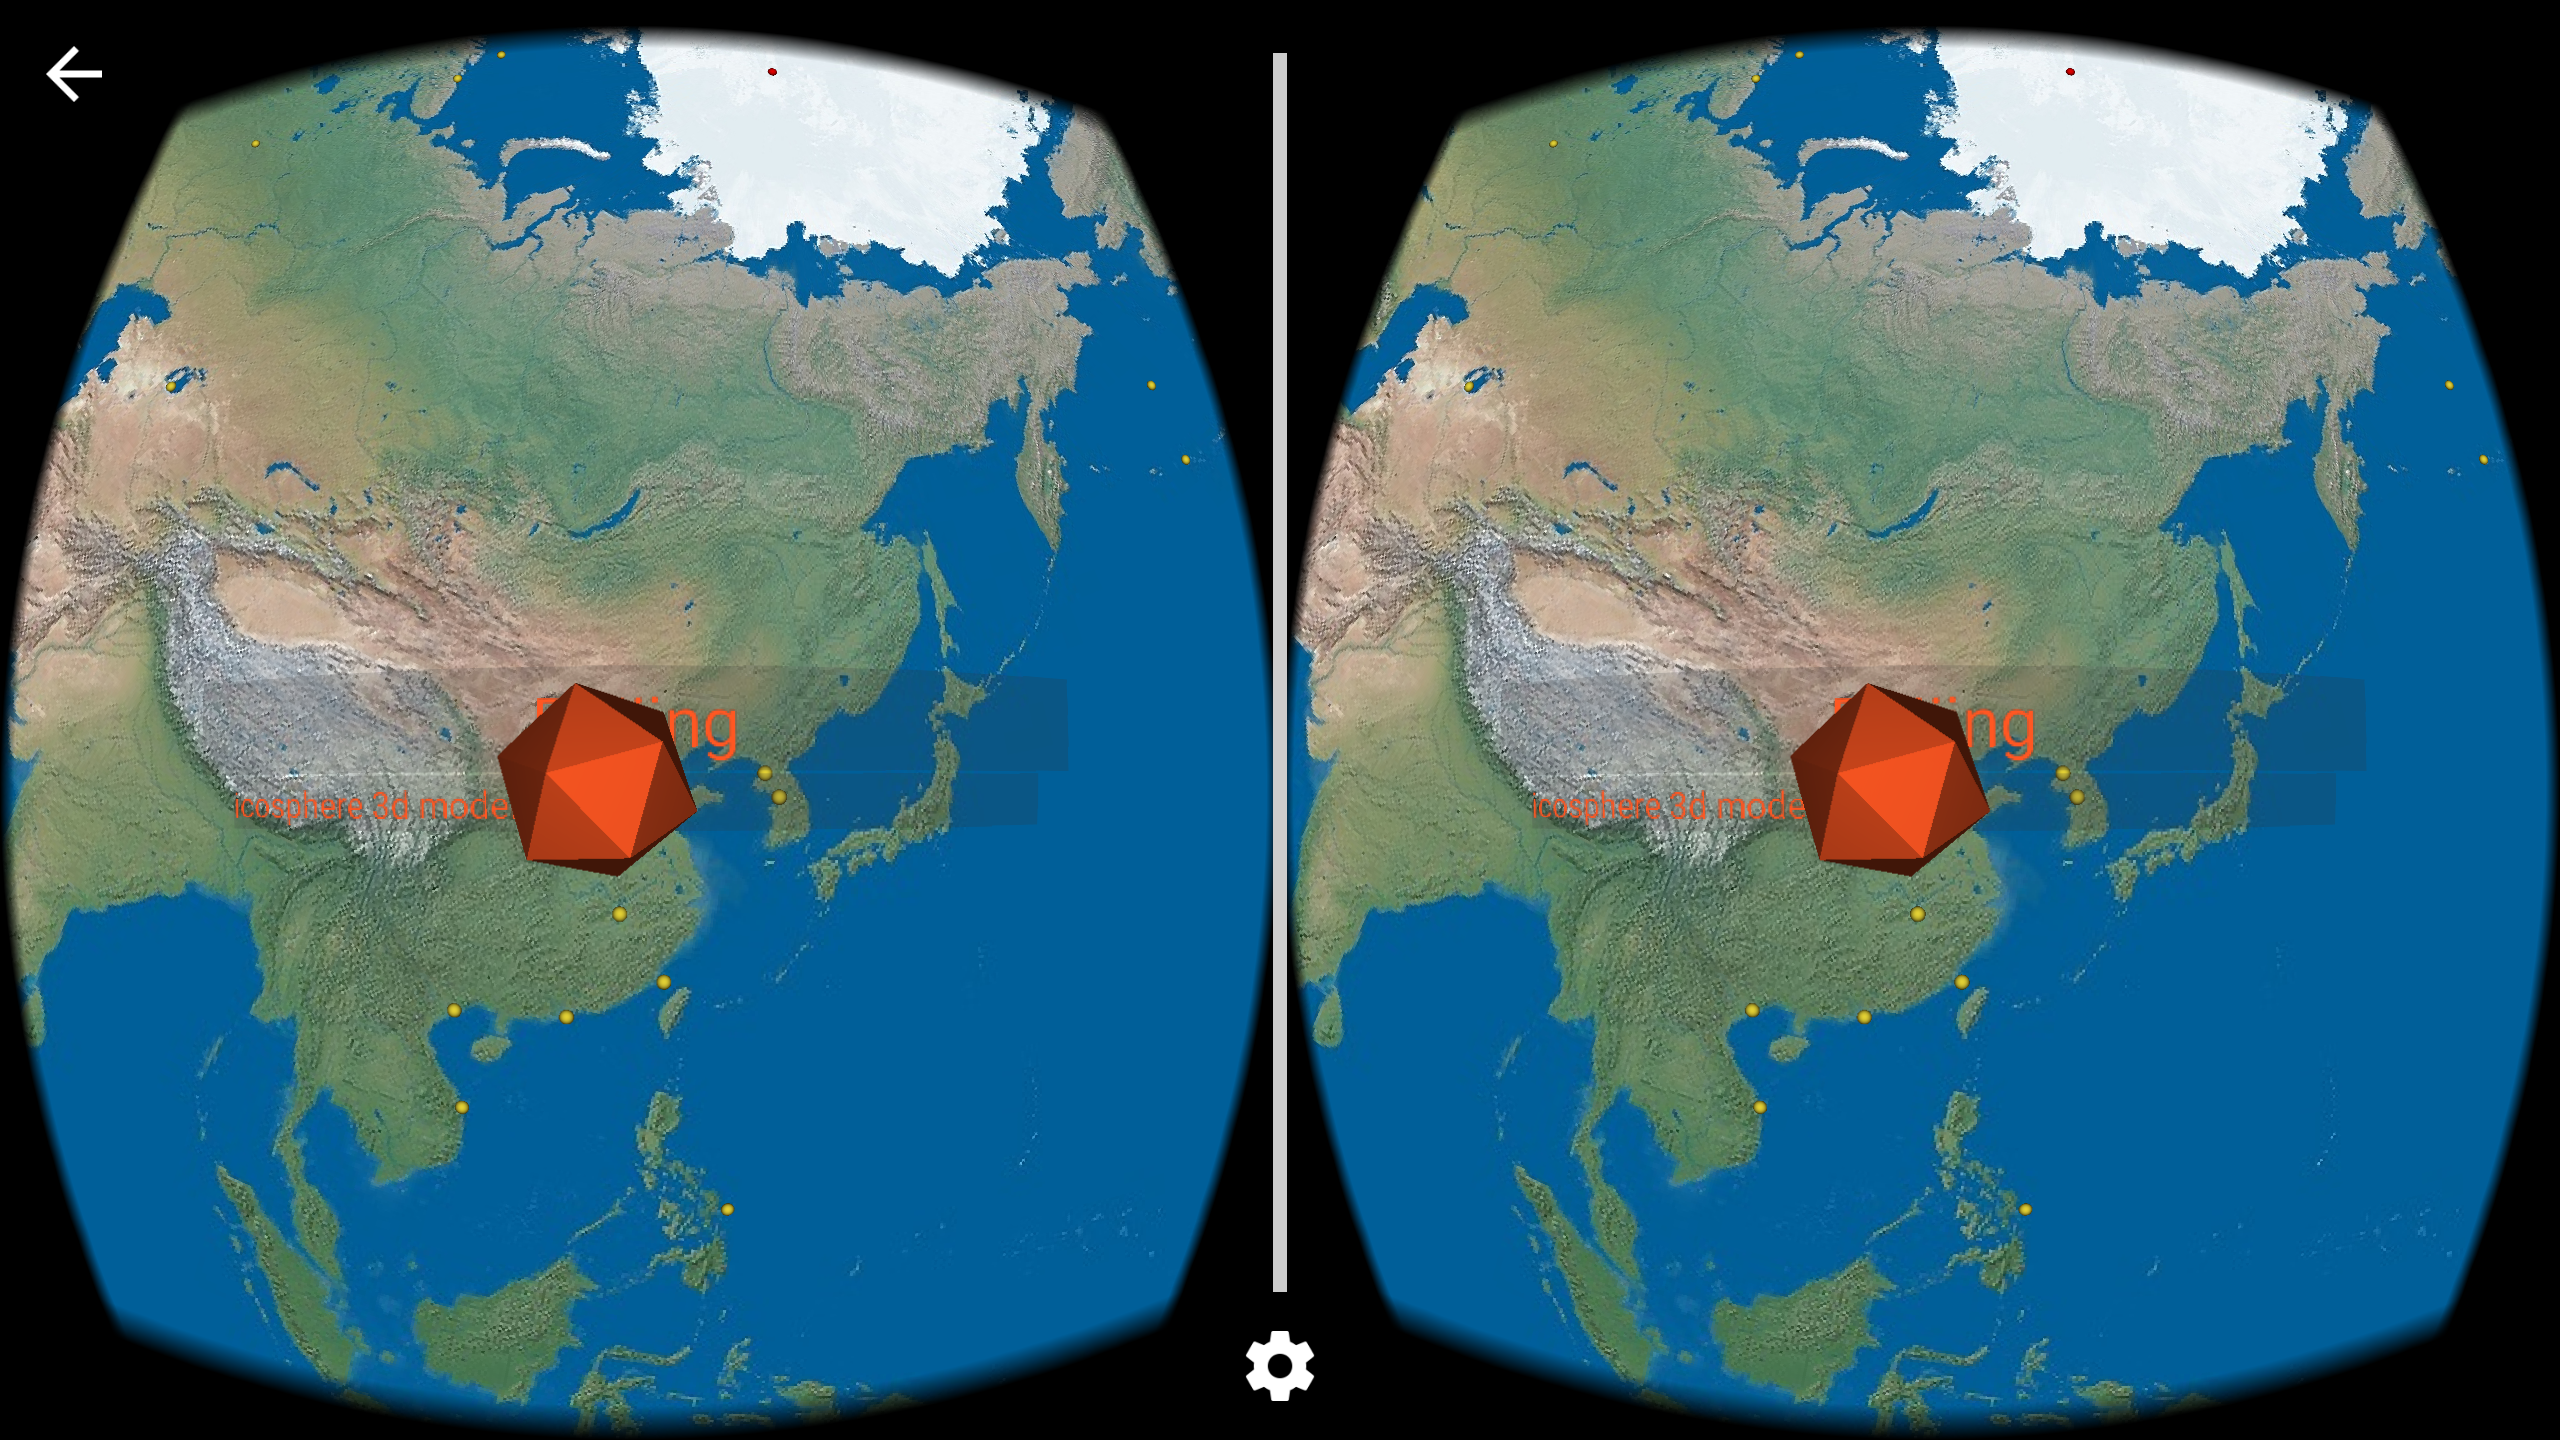
\includegraphics[width=\linewidth, keepaspectratio]{Figures/Screenshots/device-2016-10-28-012222.png}
	\decoRule
\end{figure}

\begin{figure}[H]
	\centering
	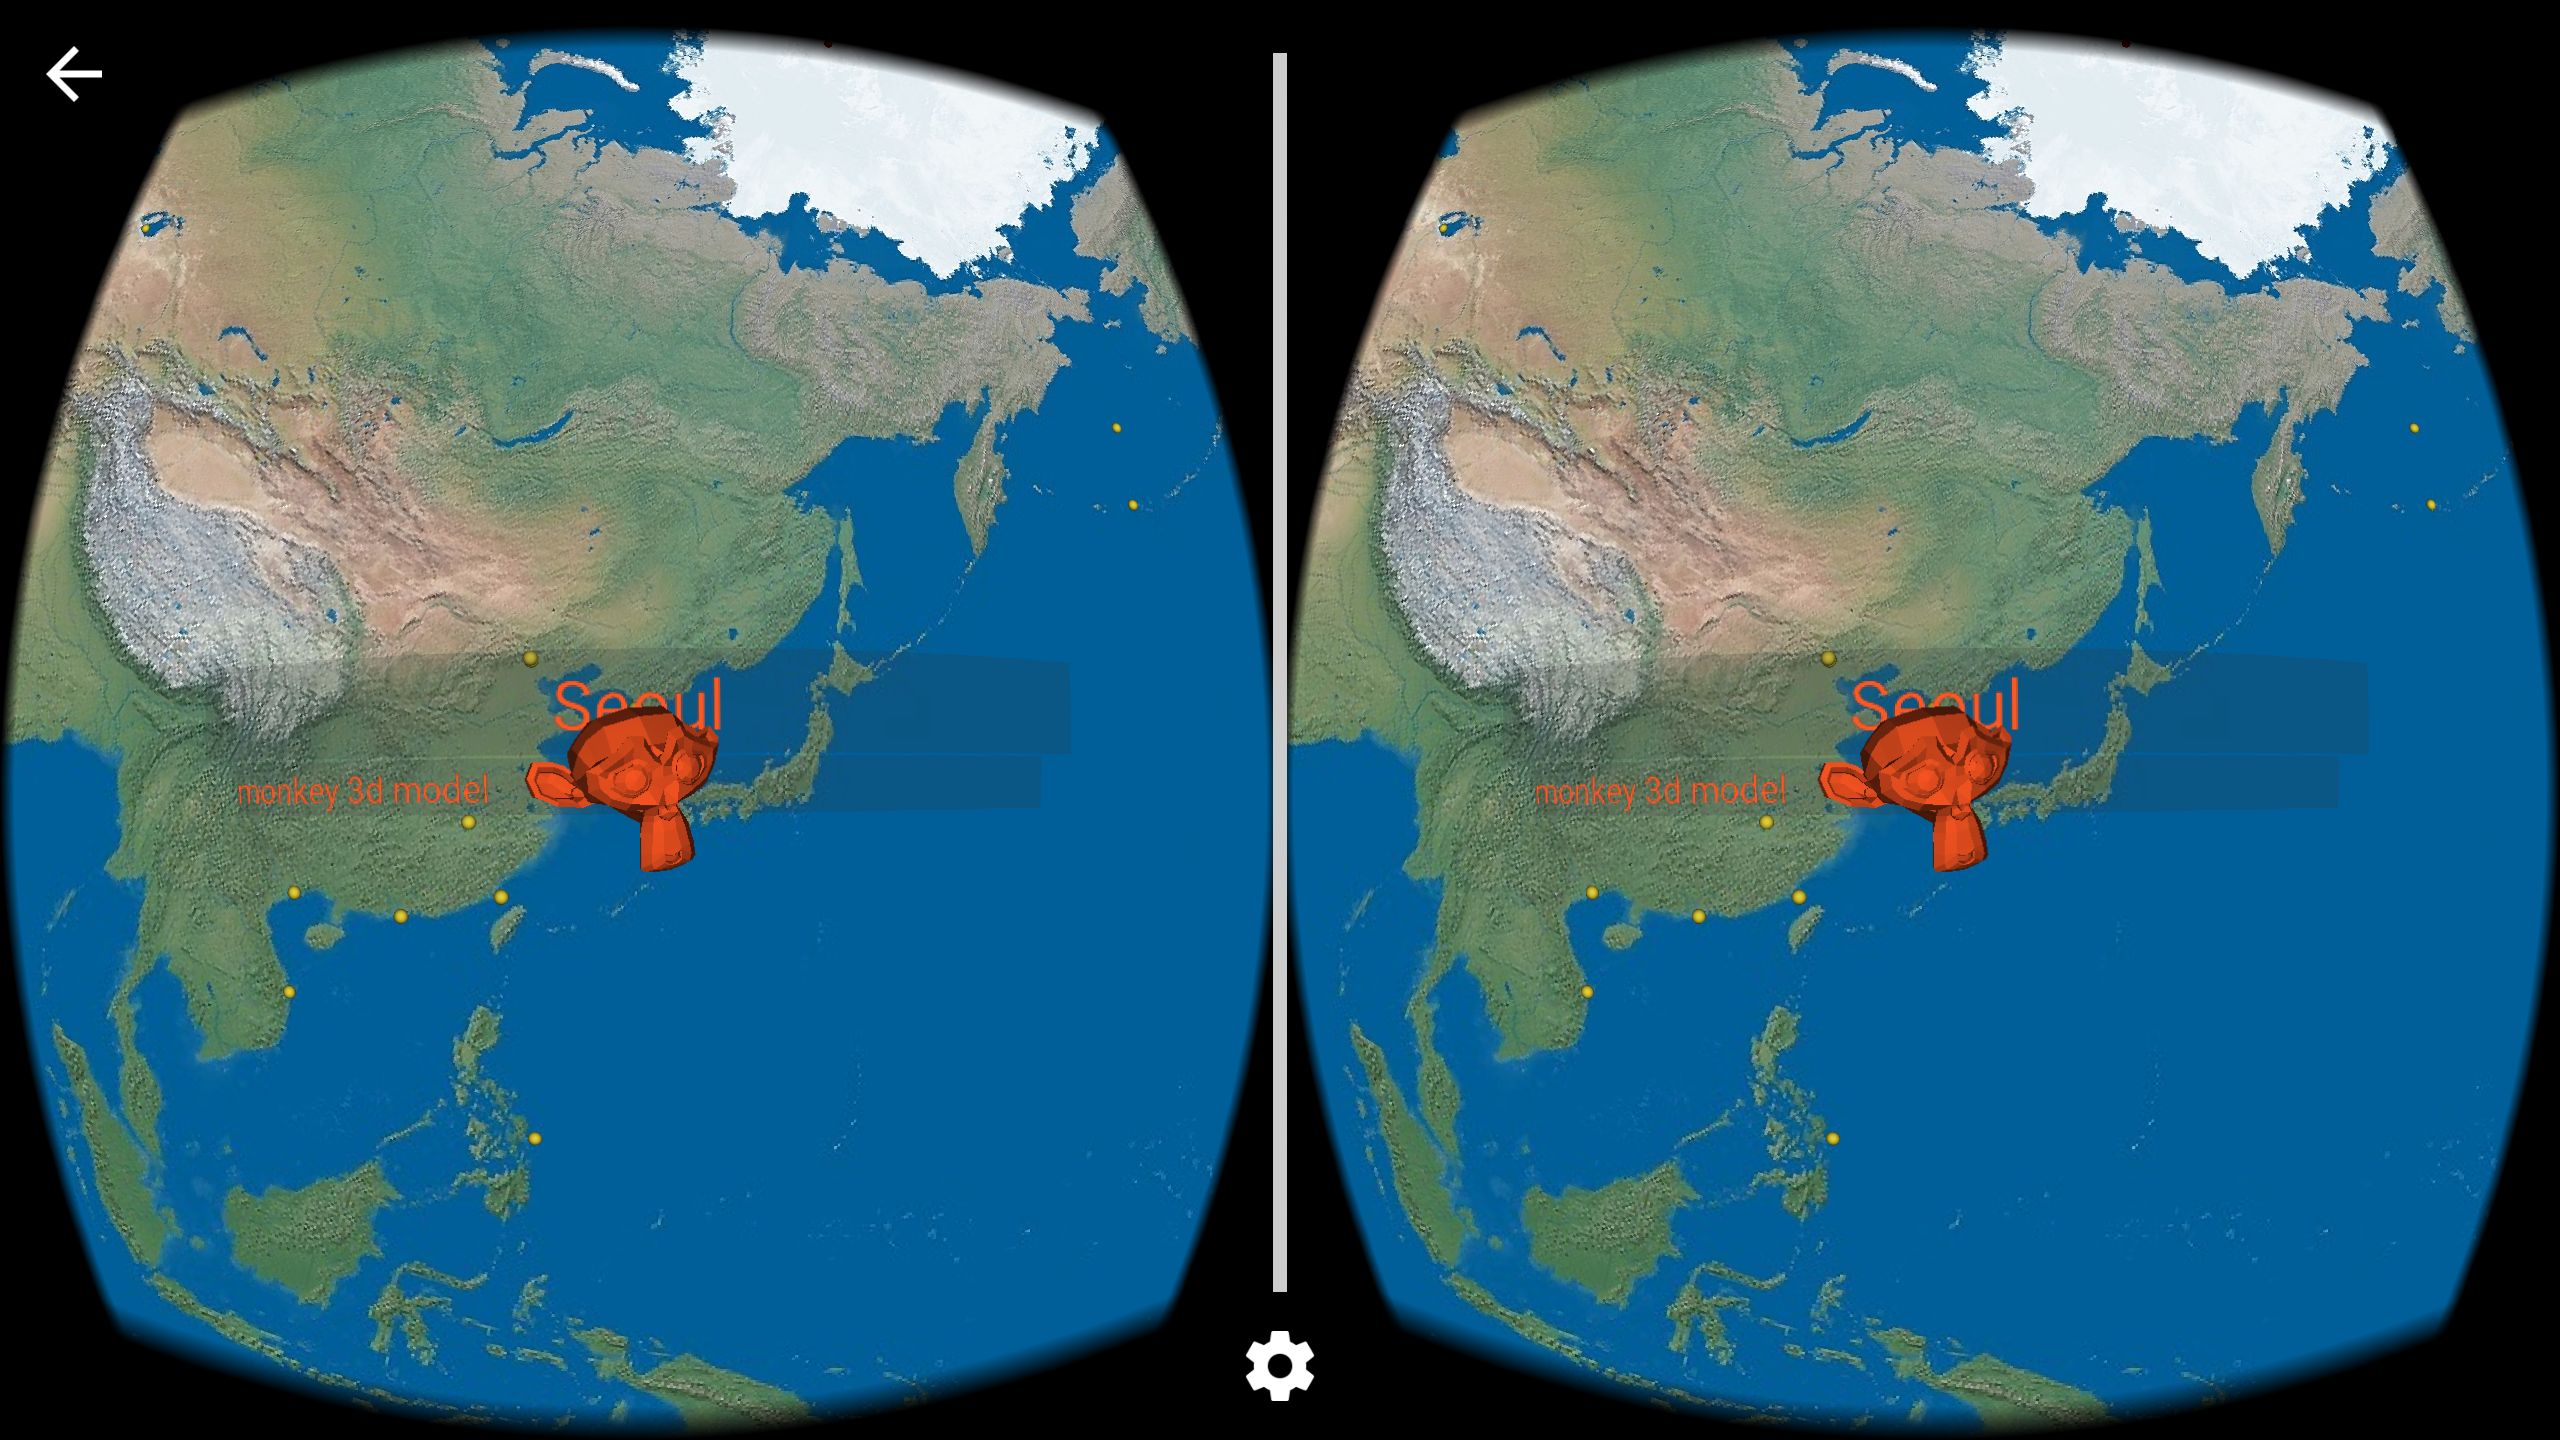
\includegraphics[width=\linewidth, keepaspectratio]{Figures/Screenshots/device-2016-10-28-012239.png}
	\decoRule
\end{figure}

\begin{figure}[H]
	\centering
	\includegraphics[width=\linewidth, keepaspectratio]{Figures/Screenshots/device-2016-10-28-012336.png}
	\decoRule
\end{figure}

\begin{figure}[H]
	\centering
	\includegraphics[width=\linewidth, keepaspectratio]{Figures/Screenshots/device-2016-10-28-012548.png}
	\decoRule
\end{figure}

\begin{figure}[H]
	\centering
	\includegraphics[width=\linewidth, keepaspectratio]{Figures/Screenshots/device-2016-10-28-012642.png}
	\decoRule
\end{figure}

\begin{figure}[H]
	\centering
	\includegraphics[width=\linewidth, keepaspectratio]{Figures/Screenshots/device-2016-10-28-012721.png}
	\decoRule
\end{figure}

\begin{figure}[H]
	\centering
	\includegraphics[width=\linewidth, keepaspectratio]{Figures/Screenshots/device-2016-10-28-013208.png}
	\decoRule
\end{figure}

\begin{figure}[H]
	\centering
	\includegraphics[width=\linewidth, keepaspectratio]{Figures/Screenshots/device-2016-10-28-013605.png}
	\decoRule
\end{figure}

%****************************************************************

\include{Appendices/appendix-kml-sample}
\include{Appendices/appendix-obj-sample}
%\end{appendices}

%****************************************************************
%	BIBLIOGRAPHY
%****************************************************************
\printbibliography[heading=bibintoc]
%\printbibliography[heading = subbibliography, title={Not Online}, nottype=online]
%\printbibliography[heading = subbibliography, title={Online}, type=online]

%****************************************************************
%	END DOCUMENT
%****************************************************************
\end{document}

%****************************************************************
